\vspace*{-0.4cm}
\section{Experimental Evaluation}
\vspace*{\subsecspace}
\label{sec:eval}


Our experimental evaluation is examines the effectiveness of our scheduling based approach for opportunistic GPU acceleration for FaaS workloads for three main metrics: i) on-GPU execution latency (which captures how efficiently we are using the hardware), ii) per-function end-to-end latency which includes the queue wait time, and iii) device utilization and throughput for hybrid CPU-GPU systems.


% Run on system with Ubuntu, 48 phys cores, Nvidia P100 GPU, 250 Gb ram
% Here we will showcase the effectiveness of our GPU memory manipulation in minimizing

\mhead{Setup and Workloads}
All experiments were run on servers running Ubuntu 20.04 on kernel version 5.4, with a 48 physical core Intel Xeon Platinum 8160 CPU with hyperthreading disabled, 250 GB of RAM, and an Nvidia V100 GPU running driver version 470.239.06. 
This isn't the latest GPU hardware, and emphasizes that our design can work with a variety of hardware, doesn't require advanced features, and is easily scalable and adaptable to other systems.


Function were sampled from Azure trace~\cite{shahrad2020serverless} in the same manner as previous works~\cite{fuerst2023iluvatar,faaslb-hpdc22}, and function frequencies are scaled using the empirical CDF of the inter arrival times, to yield workload traces of different intensities.
Based on the execution times, we select the closest matching GPU function from Table~\ref{tab:gpu-cpu} that doesn't exceed that time. 
Each experiment is run with the same trace composed of 24 functions, run for 10 minutes, and presented results are the average of 5 repeated runs.
We evaluate on multiple traces with different function mix and invocation frequency distribution, providing a wide spectrum of realistic workloads with different heterogeneity and device loads (Table~\ref{tab:scaling}).
Although \QName~is capable of enforcing per-function QoS, we set the weight of all functions to 1, for ease of exposition. 
The evaluation is presented in a top-down manner: we first analyze the end-to-end latency, then show scaling behavior, and finally investigate the effect of various \QName~parameters described earlier in Table~\ref{tab:mq-symbols}. 


% \mhead{Crossplatform verifcation on Jetson} 
% To verify correctness of our implementation across platforms, we tested it on Jetson AGX Orin, a popular edge device with an integrated Ampere Architecture GPU \cite{jetson-specs}.
% We ported GPU functions cupy, onnx-roberta, tf\_imagenet and tf\_squeezenet by rebuilding them with 
% Machine Learning Container for Jetson and JetPack (l4t-ml:r35.2.1-py3) \cite{l4tcontainer}. 
% Jetson environment had Ubuntu 20.04, L4T version 35.4.1 and JetPack version 5.1.2 setup on it with 
% driver versions 11.4.315 for CUDA, 8.6.0.166 for cuDNN and 8.5.2.2 for TensorRT.
% On tegra platforms iGPU (integrated GPU) use system memory, therefore it's not possible to overcommit and for a dGPU (discrete GPU) unified memory is not supported currently \cite{tegra-uvm}. 
% Our shim is able to intercept and replace allocation calls but it does not have any impact. 
% Therfore, our implementation works without being able to overcommit on Jetson Orin AGX.

\mhead{Scheduling Policies}
To examine the locality, fairness, and utilization tradeoff, we implement and evaluate three \emph{additional} scheduling policies in addition to our default \QName. 
% \naive~dispatches function invocations in a first-come-first-serve order and has no container pool, and represents the umoptimized baseline for black-box GPU functions. 
The second policy is \fcfs, which uses the warm pool and memory management (we move function memory on-device before executing, and move it back off after each invocation has completed).
This represents a scheduling policy with most of the important GPU optimizations, but one which is not fully locality or fairness aware.
Our third and final scheduling policy variant is \batch, which also uses all the GPU optimizations, and maximizes locality by batching invocations of each function individually.
Unlike \QName, \batch~greedily maximizes batch sizes (and hence locality) irrespective of the build-up of other functions.  
% and a \texttt{Batch} policy that separates flows and executes everything in the flow with the

Using the MQFQ design allows for easy parametrization and implementation of these and other policies for exploring the locality vs. performance tradeoff.
Both \fcfs~and \batch~use the integrated memory management and CUDA interposition shim, and thus allow us to separate out the impact of \QName's core ideas with minimal code changes and differences. 
For \fcfs, all functions are inserted into a single queue.
For \batch, we insert invocations into per-function flows, and dispatch the entire \emph{flow} containing the oldest item. % to execute all removed items serially, but prevents new items from tagging along.

%\vspace*{-0.5cm}
\subsection{GPU Scheduling Performance}
\label{sec:queue-perf}

\begin{figure*}
  \centering 
  \subfloat[\textbf{Average latency} is significantly lower with \QName~for different device-parallelism (\D) levels.  \label{fig:queue-e2e}]
  {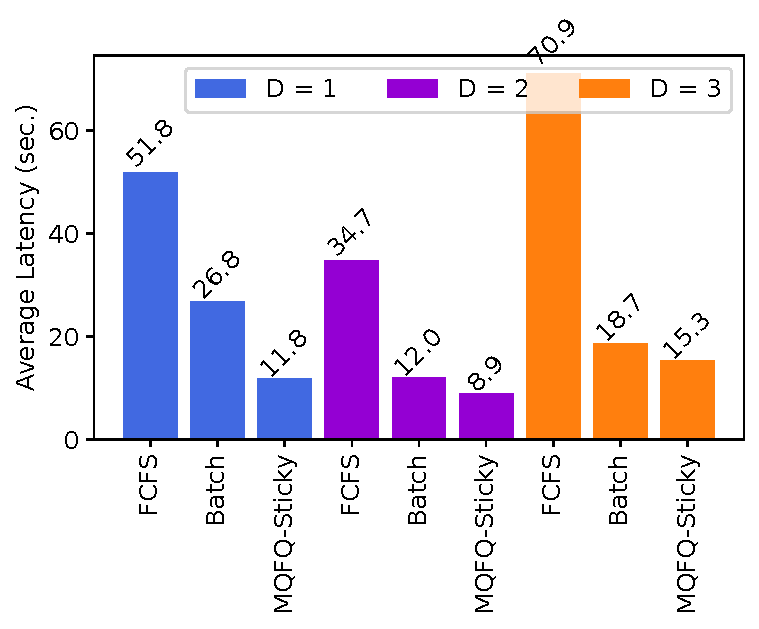
\includegraphics[width=0.32\textwidth]{../graphs/q_compare/25.7095/20/no_naive_e2e_sec.pdf}}
 \hfill  
\subfloat[The average and variance of \textbf{per-function latency} is much lower with \QName.  \label{fig:queue-fairness}]
{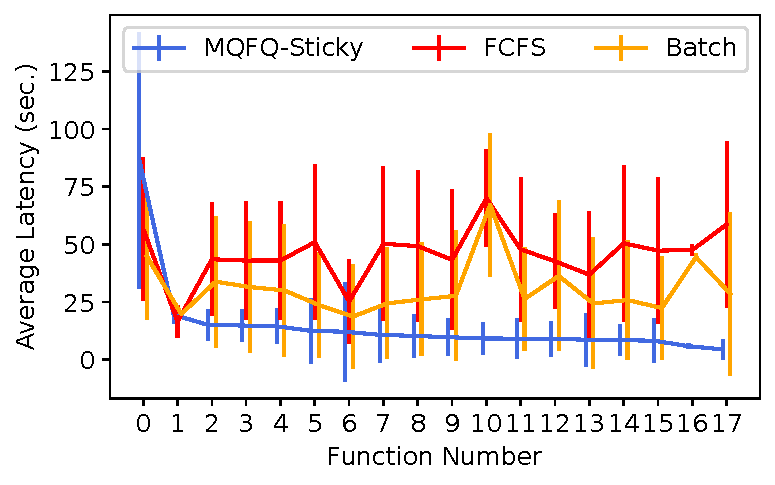
\includegraphics[width=0.35\textwidth]{../graphs/q_compare/25.7095/20/paper_fairness.pdf}}
\hfill 
\subfloat[\textbf{Device utilization} for the medium-load trace. \label{fig:util} ]
{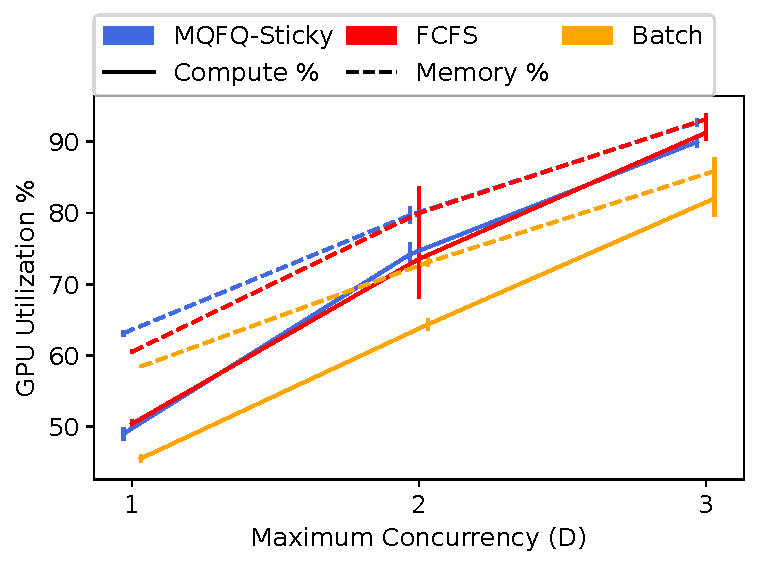
\includegraphics[width=0.3\textwidth]{../graphs/q_compare/25.7095/20/all_util_no_zeroes.pdf}}
\label{fig:base-all}
\vspace*{-7pt}
\caption{Latency, fairness, and utilization for a medium-intensity FaaS workload.}
  \vspace{\myfigspace}
% average variance across functions:
% 25.708
% mqfq,fcfs,batch
% 306.3366558710925 1775.2016313919078 1541.5163353200303
%
% 25.7095
% mqfq,fcfs,batch
% 260.76811271061183 752.4597314354334 664.7010323038504
%
% 25.707
% mqfq,fcfs,batch
% 176.98634136793837 902.0644451782704 669.7400253032657
\end{figure*}

To characterize the differences in the above scheduling policies, we first show the empirical evaluation with a \emph{medium-intensity} workload, which comprises of 24 functions with an average arrival rate of 2 invocations per second. 
This workload results in average GPU utilization of around 70\% (Figure~\ref{fig:util}), and represents the average case. 

\noindent \textbf{Average Latency.}
The latency across all invocations is shown in Figure~\ref{fig:queue-e2e}.
Not shown in the figure is the current baseline \naive~scheduling with Nvidia-docker, which does not have a container pool and suffers from excessive cold-starts.
\textbf{The \naive~average latency is close to 3,000 seconds---a $300\times$ overhead.}
The high latency is because of every invocation results in a cold-start, causing a large queue buildup.
Note that our workload trace is open-loop, and thus invocations are generated at fixed intervals.


% \naive~has extreme wait times due to cold starts caused by the lack of warm pool. 
%as we saw in Fig.~\ref{fig:container-pool-cold-hits}.
% Adding the pool and memory management in \fcfs~gives over two orders of magnitude improvement in latency, even when only a single invocation is dispatched to the GPU (D=1 case).
\QName~outperforms \fcfs~by $5\times$ with a 11.8 vs 51.8-second average respective latency thanks to its locality and fairness oriented design.
\batch~has middle of the road performance, lacking fairness and advanced locality policies.
% , and 20\% better than \batch~because it doesn't throttle functions that hog GPU time well.
% Increasing the device concurrency (\D) improves \QName~latency by a further 15\%.
For this workload, at higher concurrency levels, \QName~improves latency by an additional 25\% to an 8.9-second average per invocation.
Both competing policies also benefit from concurrency, but neither outperform \QName.
% This is caused by errant lucky items at the end of batches jumping ahead in the queue, in violation of fairness principles.
When \D~is set too high (\D=3), the device cannot handle the higher concurrency, and all policies suffer varying degrees of degradation due to resource contention and interference.
For this workload, the queuing delays account for more than 99\% of the end to end function latency, and thus scheduling policies have significant impact. 
% Execution time is equal between all three policies, as they share the GPU monitor, latency improvements come entirely from more optimal scheduling decisions and reduced cold starts.
% \todo{Add queuing vs execution split for the latency results?}

\noindent \textbf{Fairness.}
In Figure~\ref{fig:queue-fairness}, we show the per-function latency (averaged across all its invocations).
We use inter-function latency variance as our fairness metric.
\fcfs~has the worst global inter-function latency variance (752), and the highest average latency.
\QName~reduces latency in the range of $2-10\times$, and has only one-third the inter-function latency variance of \fcfs.
Also, the invocation latency variance for each function (the error bars) is $3-4\times$ lower compared with \fcfs~and \batch.

\textbf{Result:} \emph{\QName~policy provides a $5\times$ reduction in average latency across all functions, and also reduces their jitter and tail latency by $3-4\times$.}

\vspace*{\subsecspace}
\subsection{Scaling}

We now look at load, GPU, and memory scaling properties of \QName.

\begin{table}
  \caption{The latency benefit of \QName~improves with increasing GPU utilization.}
  \vspace{\captionspace}
  \label{tab:scaling}
  \begin{tabular}{rrrrr}
    GPU Util (\%) & Req/s & \QName(s) & FCFS(s) & Batch(s)\\
    \hline
    28.025 & 1.122 & 3.932 & 7.843 & 4.962\\
    35.747 & 1.797 & 2.432 & 4.511 & 2.838\\
    38.889 & 1.943 & 3.434 & 8.031 & 3.441\\
    42.740 & 1.690 & 1.046 & 1.371 & 1.054\\
    43.347 & 2.572 & 2.929 & 7.309 & 3.454\\
    52.054 & 1.125 & 2.956 & 3.512 & 2.415\\
    57.467 & 4.263 & 5.630 & 37.743 & 9.585\\
    68.141 & 2.693 & 10.543 & 44.450 & 13.570\\
    74.216 & 2.553 & 8.899 & 34.719 & 11.996\\
  \end{tabular}
  \vspace{-0.4cm}
\end{table}

\mhead{Latency vs. load}
Table~\ref{tab:scaling} shows the latency for different workload traces, each with a different mix of functions and IATs (inter arrival times), resulting in different average GPU utilization.
In general \QName~performs better at higher utilization, reducing average latency by $4-6\times$ vs. \fcfs.
When considering the latency weighted by the number of invocations, and normalized to the no-interference case, the performance gap is even higher, since smaller functions are more affected by cold-starts and unfairness in relative terms.
\QName's weighted normalized latency is more than $10\times$ lower (vs \fcfs) at higher loads, and $2.5\times$ lower vs. \batch. 


\begin{figure}
  \centering  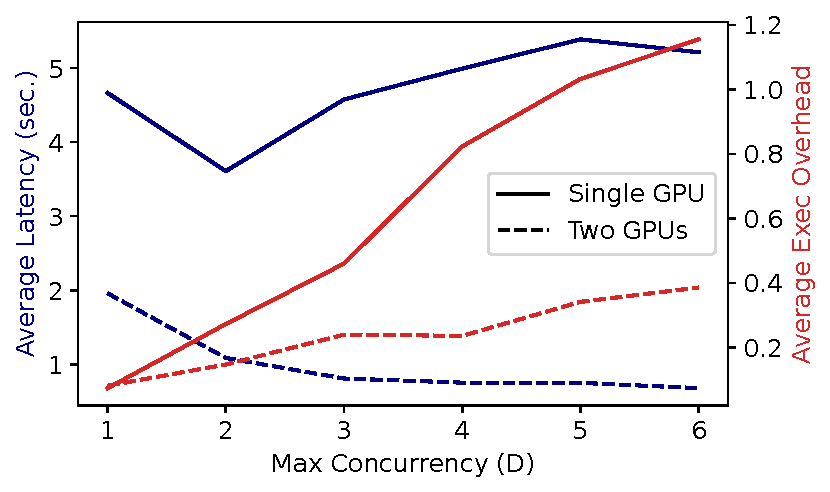
\includegraphics[width=0.35\textwidth]{../graphs/multi-gpu/25.7/concurr_scale.pdf}
  \vspace*{-8pt}
  \caption{\QName~also uses locality-aware scheduling for multiple GPUs, significantly reducing queuing.}
  \label{fig:multi-gpu}
  \vspace*{-8pt}
\end{figure}

\mhead{Multiple GPUs}
Our system easily scales to orchestrating and dispatching across multiple GPUs.
We run a high-load trace and show the comparison in Figure~\ref{fig:multi-gpu} after we add a second, identical, GPU to the server. 
% In Figure~\ref{fig:multi-gpu} we show how it adapts to running the same trace on systems with one and two identical GPUs.
Two GPUs not only allows us to run $\D\times2$ invocations, but also do on-the-fly load balancing between them to avoid compute contention with higher \D. 
% and therefore expect a corresponding 2x performance improvement.
As a baseline, the multi-GPU blue dashed line has $2.3\times$ lower latency at \D=1.
At higher device parallelism, the multi-GPU case sees a latency reduction of $4\times$ vs. the single GPU setting. 
Device parallelism also slightly increases the execution overhead due to interference, but is offset by the smaller queues. 

% Scaling \D~to 6, we see reductions in latency up to \emph{87\%} -- whereas the single device is quickly overloaded and has worse overall performance.
% % This balancing boosts latency reduction to \emph{87\%} when \D~is very high
% % , much better than our expected linear speedup.
% Execution overhead in red increases dramatically with \D~when only one GPU is available, in the worst case a nearly 6x increase.
% % With higher \D, our dispatches also load balance between the two devices, something not possible in the solitary device case.
% However, with two GPUs in the red dashed line, once $\D \ge 2$ the load balancing mitigation lowers overhead by 45\%, and a maximum of 66\%.
% Reduction of this overhead is a significant contributor to lower latencies as well.
% The ability to choose devices results in a 70\% reduction in execution overhead, entirely from mitigating compute overloading.



% e2e
% [4.663137860034904, 3.607658436985101, 4.575037657122783, 4.991578333097969, 5.386245616200919, 5.212470496279234]
% [1.9581354786418401, 1.0854709685368538, 0.8082406824696803, 0.7523517956355057, 0.7496512471943295, 0.677325266114725]
% [0.58008201 0.69912036 0.82333682 0.84927577 0.86082119 0.87005677]
% exec
% [0.07375773205618323, 0.27254631424617926, 0.4598690614061698, 0.8230379144178025, 1.0323527250435014, 1.154964442968281]
% [0.08146243318283061, 0.14722147302861147, 0.2398143374961277, 0.2358641959639591, 0.341338564858076, 0.3858309500976596]
% [-0.10445957  0.45982952  0.47851604  0.71342244  0.66935859  0.66593695]


\begin{table}
  \centering
  \caption{Hybrid CPU+GPU reduces latency by more than 2x compared to CPU-only and GPU-only execution.}
  \vspace{\captionspace}
  \label{tab:cpu-gpu}
  \begin{tabular}{|l|r|}
  \hline
  Case & Avg. latency (s) \\ \hline
  CPU-only & 2.03 \\
  1 GPU & 3.43 \\
  2 GPUs & 1.08 \\
  CPU+GPU & 1.00 \\
  \hline 
\end{tabular}
\vspace{-0.4cm}
\end{table}

\mhead{Hybrid CPU+GPU execution}
For evaluating hybrid execution, we use a GPU-speedup based dispatch policy.
We use offline profiling to obtain the GPU speedup for functions, and only run the top 50 percentile of functions on GPU, and rest use the CPU.
This corresponds to functions having GPU speedup of $>3\times$ being eligible for GPU acceleration. 
Other functions avoid queuing for the GPU and run immediately on the system's plentiful 48 CPU cores. 
The average function latencies are shown in Table~\ref{tab:cpu-gpu} for a high-intensity workload. 
Due to excessive queuing and contention, a single GPU degrades latency by 38\%. Adding a second GPU alleviates this load and reduces latency by half.
Interestingly, hybrid execution with the CPU and single GPU reduces latency even further, thus showing the benefits of heterogeneous hardware for FaaS workloads. 

% CPU 2.030147525728988
% GPU 3.4336443728988
% Two GPUs 1.0899518145507185
% CPU/GPU 0.9972267068610635


\begin{figure}
  \centering  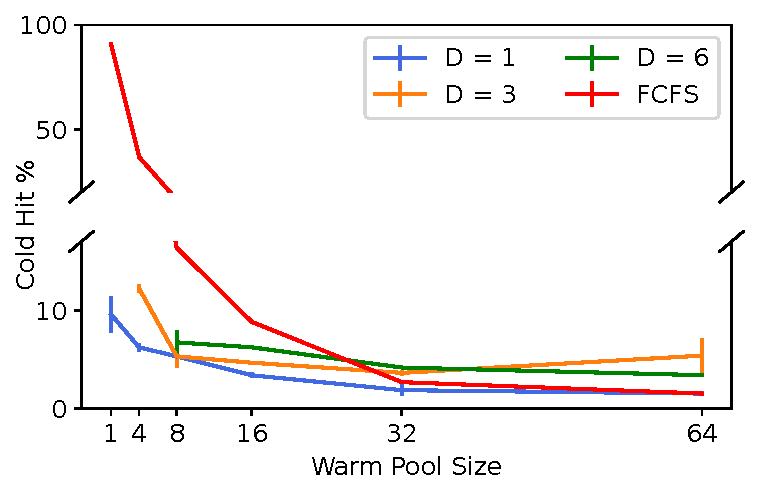
\includegraphics[width=0.30\textwidth]{../graphs/container_pool/big-60min/65/cold_hits.pdf}
  \vspace*{-8pt}
  \caption{Container-pool reduces cold-starts. \QName~provides higher locality.}
  \vspace*{-14pt}
  \label{fig:caching}
\end{figure}

\mhead{Container Pool Size}
% Functions running warm is vital for low latency in serverless systems which, and our UVM shim enables maintaining a warm pool of GPU containers.
For temporal locality, the invocation patterns and batching plays a key role in reducing cold starts.
The performance difference between \QName~and \fcfs~can be largely attributed to the cold-hit ratio of the invocations.
Figure~\ref{fig:caching} shows the \quotes{miss-rate curves} for the medium-intensity trace as we increase the number of containers in our container pool.
We focus on the number of containers in the pool, rather than MB of pool memory for simplicity.
Idle containers do take up CPU memory, and work managing the memory used by caching containers is orthogonal to our design~\cite{faascache-asplos21}.
Since \QName~prefers smaller batches of functions and does anticipatory keep-alive, it has a high temporal locality and its cold-hit \% is in the range of 2-8\% across a range of pool sizes and device concurrency.
In contrast, \fcfs~has 50\% cold-starts with a pool size of 4, and achieves parity with \QName~only at largest pool sizes when the popular functions can fit in the container cache.


\vspace*{\subsecspace}
\subsection{Impact of Scheduling Parameters}
\label{sec:queue-knobs}

In this subsection, we explore the effects of configuration knobs to see their effect on performance, which also sheds a light on the empirical relationships between fundamental parameters of locality and throughput. 


% \begin{figure}
%   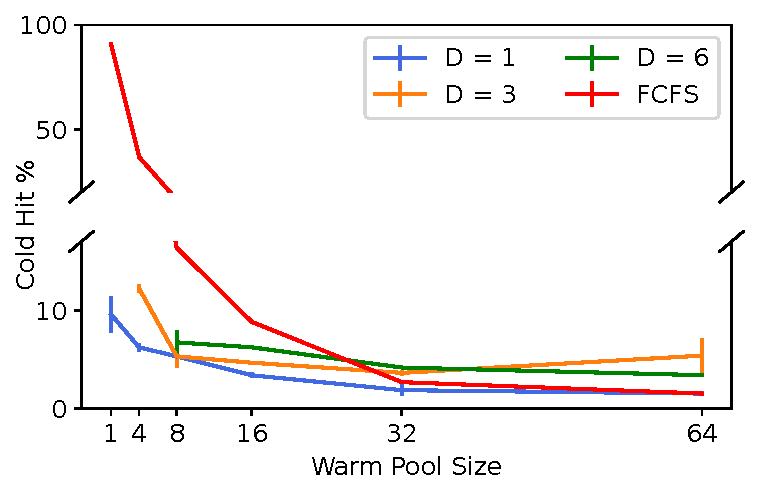
\includegraphics[width=0.4\textwidth]{../graphs/container_pool/big-60min/65/cold_hits.pdf}
%   \vspace*{\captionspace}
%   \caption{\QName~greatly reduces cold hits compared to FCFS, and is improved with a large container pool size. 
%           More cold hits are also caused when \D~(concurrency) is raised, needing private containers to serve concurrent invocations.}
%     \label{fig:container-pool-cold-hits}
%     \vspace{-0.4cm}
% \end{figure}

\begin{figure}
  \centering
  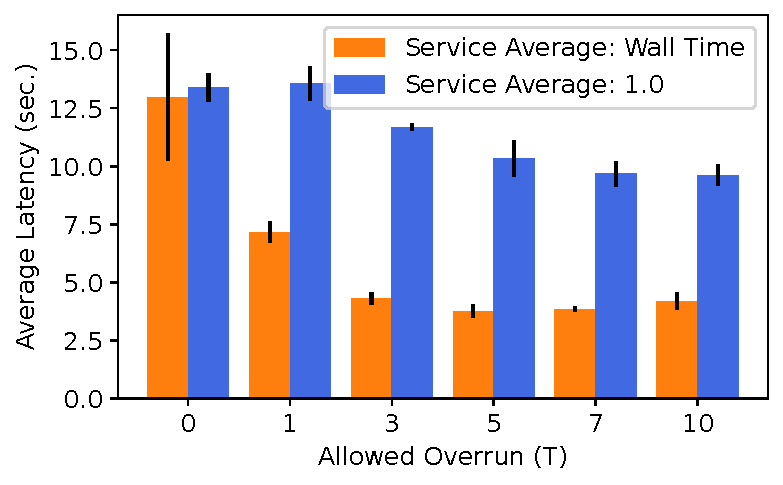
\includegraphics[width=0.3\textwidth]{../graphs/unfairness/25.7/e2e_sec.pdf} 
  \vspace*{-5pt}
  \caption{Larger T yields more batching and lower latencies because it allows popular flows to run ahead. Using historical function execution latencies helps significantly compared to uniform flow costs in classical fair queuing.}
  \label{fig:T-service}
    \vspace*{-7pt}
\end{figure}

\mhead{Flow over-run (\T)}
Recall that flow virtual times are within \T~of each other.
Larger \T~results in more locality and batching opportunities, but decrease fairness, since flows may get to monopolize resources for longer before being throttled.
Figure~\ref{fig:T-service} shows the average latency decreasing, but with diminishing returns, as the over-run is increased. 
The figure also shows the value of using function wall clock execution times.
When all flow usages are assumed to be constant (1.0 in the figure), long functions may dominate, which increases average latency by more than 3x.
\emph{Thus, a small amount of over-run guided by function characteristics helps significantly.}

\begin{figure*}
  \centering
  \subfloat[Anticipatory flow keep-alive (non-zero flow TTL) can reduce latency by up to 50\%. We use function IAT for scaling the TTL. \label{fig:flow-ttl}]
  {  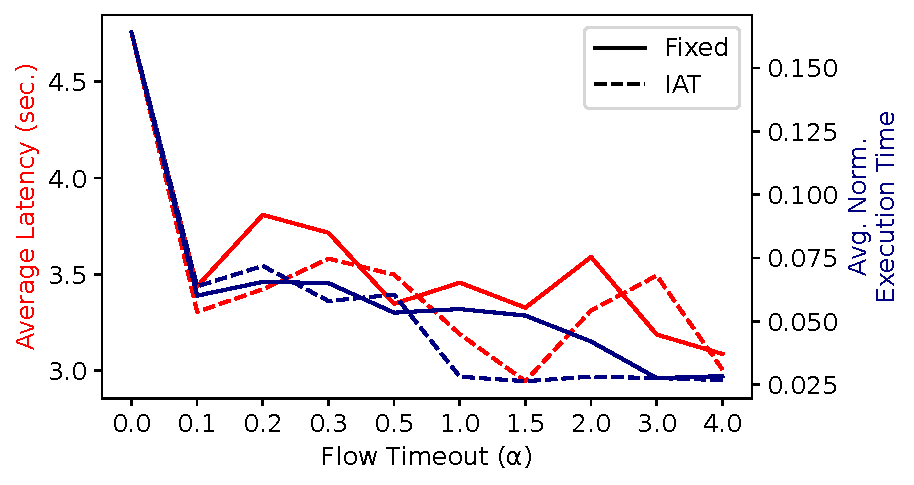
\includegraphics[width=0.35\textwidth]{../graphs/ttl/25.8/mqfq-ttl-compare.pdf}}
  \hfill
  \subfloat[Concurrent function invocations (\D) increase execution time due to contention. GPU utilization thresholds reduce overload. \label{fig:concur-exec-overhead}]
  {  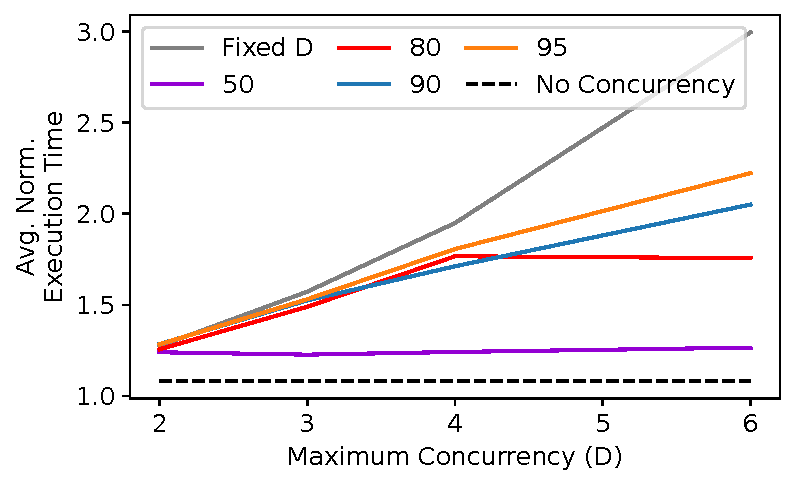
\includegraphics[width=0.3\textwidth]{../graphs/concurrency/25.7/paper_exec_overhead.pdf}}
  \hfill 
  \subfloat[Concurrent execution can reduce latency by reducing queuing. However, this is negated by execution interference  at higher levels.  \label{fig:concur-e2e}]
  {  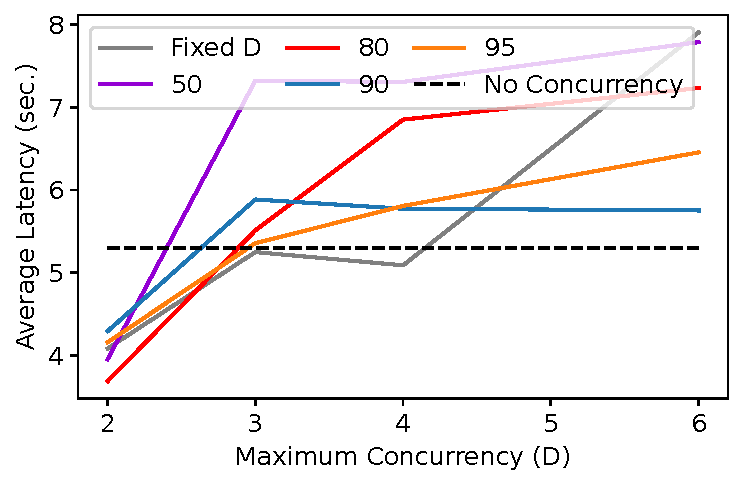
\includegraphics[width=0.3\textwidth]{../graphs/concurrency/25.7/paper_e2e_sec.pdf}}
  \vspace{\captionspace}
  \caption{Flow TTL and device parallelism (\D) are set based on workload and utilization.}
  \vspace{\captionspace}
  \label{fig:knobs-all}
\end{figure*}


\mhead{Flow keep-alive TTL}
Empty flows remain active until a TTL expires, after which they're made inactive and have their resources evicted.
Figure~\ref{fig:flow-ttl} shows the improvement to both execution time as compared to ideal warm performance and latency as the TTL grows.
The execution overhead is reduced because of warm start locality, and is the main factor behind latency reduction. 
Setting any global TTL (the solid line), at even a small 0.1 seconds, improves latency and overhead by 25\% and 50\% respectively. 
% Latency sees a 25\% improvement and execution time over 50\%, from \emph{any} TTL policy, and 
Increasing the TTL to up to 4 seconds sees significant, but diminishing, returns.


%For the \texttt{Fixed} line, the X axis represents time in seconds for the global TTL.
%For the \texttt{IAT} line, the X axis represents the factor by which each function's IAT was scaled to become its TTL.

% A large 4 second time can reduce latency by 35\% and execution time by 40\%.

By default, we base TTL on each function's inter-arrival-time (IAT), rather than have a global fixed time.
This method sets the TTL for each flow to the IAT multiplied by the value ($\alpha$) on the X axis, plotted as the dashed line.
For flow timeout ($\alpha$), our default range is between 1 and 2, which contains the minima, as shown for this particular trace (at 1.5).
Higher TTLs ($\alpha > 3$) may result in too many active functions and pressure on the container pool. However, our design is robust to very large TTLs: the pool uses LRU eviction and the resulting impact on performance even at high TTLs is low.
\emph{Thus, anticipatory scheduling improves latency by 50\%, and \QName~performance is not sensitive to the TTL.} 


\mhead{Device Concurrency}
We now explore the tradeoff due to device concurrency, which can improve utilization, but also risks performance interference and is dependent on the co-located applications, which are constantly changing in FaaS workloads. 
We run our medium workload and adjust device concurrency using \D~and examine the effect on execution time (without considering queuing delays) in Figure~\ref{fig:concur-exec-overhead}. 
% Figure~\ref{fig:concur-exec-overhead} examines the effect on execution overhead as the concurrency \D~is changed and is made dynamic.
All numbers are normalized to the no concurrency (i.e. $\D=1$) case. 
When we increase \D~and use a fixed value, shown in the gray line, we always have \D~number of invocations trying to execute on the GPU concurrently.
Normalized execution time is unsurprisingly correlated with \D, as GPU contention between invocations causes up to 100\% overhead at the maximum $\D=6$.


By default, we use the GPU utilization upper bound (shown by different lines in Figure\ref{fig:concur-exec-overhead}).
Setting the upper bound to 50\% utilization prevents over-saturation of the GPU, and reduces overheads significantly. 
However, this increases the queuing and total latency, as shown in Figure~\ref{fig:concur-e2e}.
For this workload, the total latency increases slightly due to contention and interference, and the limited memory of our GPU (16 GB).
The ``sweet spot'' is $\D==2$, and latency increases slightly by 30\% at higher levels.
Our present design leaves the maximum \D~to the operator, since the utilization based capping dampens its effect. 
\emph{Thus, allowing concurrent dispatch to the GPU, controlled to minimize contention, significantly improves global latency and utilization of the device.}

\textbf{Result:} \emph{Our introduced features such as flow over-run, anticipatory scheduling, utilization-driven concurrency, all contribute to latency reduction by $1.5-3\times$. A wide range of these parameters yield similar performance, making our system robust, yet still providing operators enough flexibility for fine-tuning based on workloads and operational requirements.}

\begin{comment}
% The remaining lines represent the GPU utilization percentage at which we dynamically adjust \D~but have a fixed maximum (\Dmax), represented by the X axis value.
In the remaining lines when we adjusted \D~dynamically with utilization as described in Section~\ref{sec:mq}, at varying thresholds.
For example the purple line limits \D~at 50\% utilization, and given this low number, does not see an increase in execution time because it refuses to dispatch, despite a growing maximum \D.
% The other utilization points allow more concurrent dispatches, and see increased execution times.
The 80\% line has a minor 1.2x normalized execution time, equal to that of 50\%, but reaches a higher plateaus with large \D.
Next we show the effect controlling \D~has on latency.
% all are more limited
% In the dynamic case, when the compute utilization is below 95\%, we increase \D~and dispatch a new invocation.
% \D~is capped by a maximum configuration setting to prevent runaway dispatching that can occur during time in between active function's kernel launches.
% All see a small increase in overhead when $\Dmax==2$, equal between all values.
% A low percentage such as 50\% has stable overhead close to that of when $\D==1$, but at the expense of high queuing time due to lack of dispatches.
% Higher \Dmax~sees them separate but reach a plateau of maximum overhead, as the GPU manager limits \D~as it detects high device contention.

% Execution time isn't the only metric impacted, 
% Latency for invocations is affected by \D, throughput at the expense of individual invocation execution time.
Latency in Figure~\ref{fig:concur-e2e} changes with \D, throughput at the expense of individual invocation execution time.
Both fixed and dynamic methods have roughly 20\% better latency than when concurrency is disabled, with our 80\% line improving by 30\%.
The minor increase in execution time from concurrency at this point is outweighed by throughput gains.
Setting \D~too large eliminates this gain by offsetting it with the high execution time overheads we saw previously, or long waiting periods for usage to reduce, shown in the 50\% line case.
% is decreased across the board when $\Dmax==2$, and nearly 20\% better than baseline when utilization monitoring is at 80\%.
These are similar to the results in Fig.~\ref{fig:queue-e2e} which used a different trace, showing that the effect of \D~can vary with the function makeup of load.
Allowing concurrent dispatch to the GPU, controlled to minimize contention, significantly improves global latency and utilization of the device.
% This trend does not continue, caused by queuing at the conservative level of 50\% and encroaching execution overhead at higher levels.
% The scalability of \D~hinges on a variety of factors: function workload composition, device compute capability, and device memory size.
% Larger devices can support more functions, but this can be offset by an equally expensive function to run.

\end{comment}

% There is nothing wrong with the graph. Fixed D is only better than the dynamic options at D==3 and D==4 for latency
% It has worse execution overhead at all these points.
% It also has worse latency at _all_ points D>2 than having NO concurrency (the dashed line)
% \{Investigate/fix the avg latency vs. D graph. Fixed D does best? Maybe keeping the exec overhead graph will suffice.}


%%% Local Variables:
%%% mode: latex
%%% TeX-master: "paper"
%%% End:
